%%% File encoding: UTF-8
%%% äöüÄÖÜß  <-- keine deutschen Umlaute hier? UTF-faehigen Editor verwenden!

%%% Magic Comments zum Setzen der korrekten Parameter in kompatiblen IDEs
% !TeX encoding = utf8
% !TeX program = pdflatex 
% !TeX spellcheck = de_DE

\documentclass[12pt, letterpaper]{article}

%----------------------------------------------------------------------------------------
%	PACKAGES AND OTHER DOCUMENT CONFIGURATIONS
%----------------------------------------------------------------------------------------

\usepackage[a4paper,left=2.5cm,right=2cm,top=2.5cm,bottom=2.5cm]{geometry}
\usepackage[utf8x]{inputenc}
\usepackage[german]{babel}
\usepackage{graphicx}
\usepackage{caption}
\usepackage{minted} %code
\usepackage{amsmath}
\usepackage[colorinlistoftodos]{todonotes}
\usepackage{fancyhdr}
\usepackage{hyperref}
\usepackage{mathpazo} % Palatino font
\usepackage{float}

%----------------------------------------------------------------------------------------
% SETUP
%----------------------------------------------------------------------------------------

\hypersetup{
    colorlinks,
    citecolor=black,
    filecolor=black,
    linkcolor=black,
    urlcolor=black
}

\pagestyle{fancy}
\fancyhf{}
\rhead{Englisch - Roither}
\lhead{SWK5-WETR}
\rfoot{Seite \thepage}
 
\setminted[]{
	frame=single,
	breaklines,
	samepage=false
} 

\usemintedstyle{csharp}

\graphicspath{ {pictures/} }

%----------------------------------------------------------------------------------------
% COMMANDS
%----------------------------------------------------------------------------------------

\newcommand{\img}[3] {
\begin{figure}[H]
	\centering
	\includegraphics[width=#3\linewidth]{#1}
	\caption{#2}
\end{figure}
}

 
%----------------------------------------------------------------------------------------
% BEGIN
%----------------------------------------------------------------------------------------

\begin{document}

%----------------------------------------------------------------------------------------
%	TITLE PAGE
%----------------------------------------------------------------------------------------

\begin{titlepage} % Suppresses displaying the page number on the title page and the subsequent page counts as page 1
\newcommand{\HRule}{\rule{\linewidth}{0.5mm}} % Defines a new command for the horizontal lines, change thickness here

\center % Center everything on the page
 
%----------------------------------------------------------------------------------------
%	HEADING SECTIONS
%----------------------------------------------------------------------------------------

\textsc{\LARGE FH Hagenberg}\\[1.5cm] % Name of your university/college
\textsc{\Large Projektarbeit}\\[0.5cm] % Major heading such as course name
%\textsc{\large Minor Heading}\\[0.5cm] % Minor heading such as course title

%----------------------------------------------------------------------------------------
%	TITLE SECTION
%----------------------------------------------------------------------------------------

\HRule \\[0.4cm]
{ \huge \bfseries Weather Tracer - Dokumentation}\\[0.4cm] % Title of your document
\HRule \\[1.5cm]
 
%----------------------------------------------------------------------------------------
%	AUTHOR SECTION
%----------------------------------------------------------------------------------------

\begin{minipage}{0.9\textwidth}
\begin{flushleft} \large
\emph{Autor:}\\
Daniel \textsc{Englisch}\\ % Your name
Andreas \textsc{Roither} % next name
\end{flushleft}
\end{minipage}

\begin{minipage}{0.9\textwidth}
\begin{flushright} \large
\emph{Übungsleiter:} \\
Daniel \textsc{Sklenitzka} % Supervisor's Name
\end{flushright}
\end{minipage}\\[2cm]


{\large \today}\\[1cm] 
{Finale Ausbaustufe}\\[2cm]



\includegraphics[scale=0.25]{logo.png}
 
%----------------------------------------------------------------------------------------

\vfill % Fill the rest of the page with whitespace

\end{titlepage}

%----------------------------------------------------------------------------------------

\tableofcontents

\section{UI Sketches}
\setlength{\parindent}{0ex}
\subsection{Simulator}

Die Navigation im Simulator ist in vier Schritte eingeteilt:
\begin{itemize}
    \item Auswählen von zu simulierenden Stationen
    \item Erstellen von Generierungspresets
    \item Zuweisen dieser Presets zu den einzelnen Stationen
    \item Simulieren der Messdatengenerierung mit Live-Visualisierung
\end{itemize}

Die einzelnen Stages werden mithilfe eines Tab-Controlls umgesetzt und man kann jederzeit, wenn die Simulation gestoppt ist, Einstellungen vornehmen.

\subsubsection{Stationen auswählen}

Alle verfügbaren Stationen werden in der rechten Liste (siehe Abbildung \ref{fig:sketch_select_station}) angezeigt. Es ist für beide Spalten möglich, den Inhalt mit der sich oberhalb befindlichen Filtereingabe zu filtern, wobei auf mehrere Eigenschaften einer Station (Name, Postleitzahl, Besitzer, etc.) gefiltert wird. Die Pfeile zwischen den Spalten dienen nur zu visuellen Betonung, dass die Stationen per Mausklick von der einen Spalte in die andere verschoben werden können. Nachdem alle zu simulierenden Stationen ausgewählt wurden, kann man entweder durch Klicken des \grqq Weiter\glqq-Buttons oder durch Auswählen des nächsten Tabs zum nächsten Schritt gewechselt werden.

\begin{figure}[H]
\centering
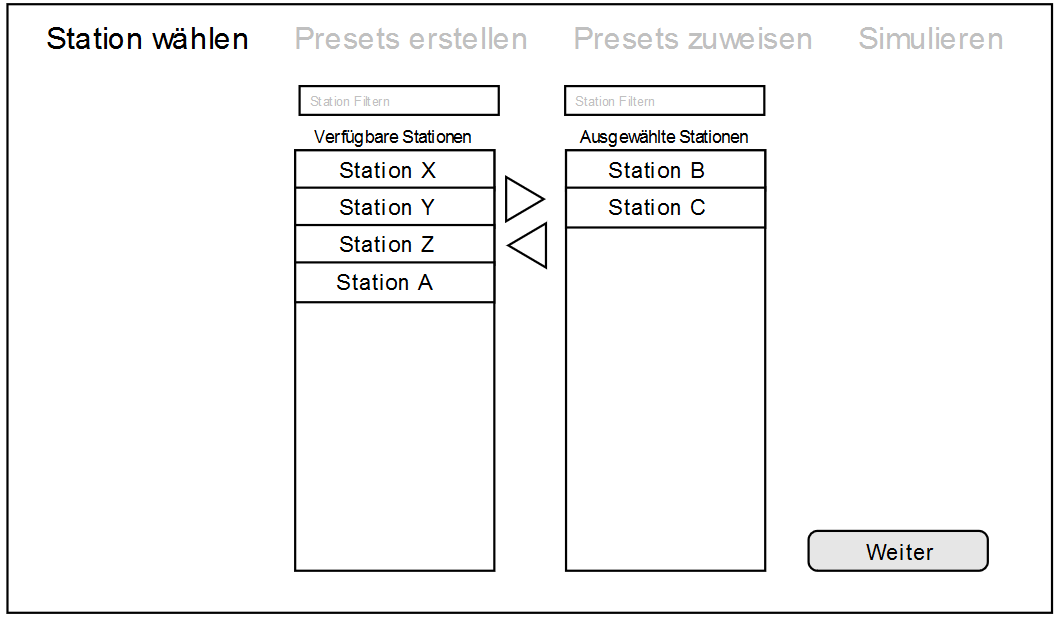
\includegraphics[width=1\textwidth]{pictures/sketches/simulator/select_sataion.png}
\caption{UI Sketch für das Auswählen von Stationen}
\label{fig:sketch_select_station}
\end{figure}
\raggedright

\subsubsection{Preset erstellen}

Um ein Preset zu erstellen muss zunächst in die korrespondierenden Felder diverse Daten eingegeben werden. Für  Minimalwert und Maximalwert bzw. Presetname wurden einfache Textfelder verwendet. Die Eingabe des Beginn- und Enddatums erfolgt durch ein Datetime Feld. Der Typ der zu generierende Messdaten, die Art der Verteilung und die Frequenz der Erstellung des Presets wird, wie in Abbildung \ref{fig:sketch_add_preset} zu sehen, mit Dropdowns festgelegt. Wenn alle Presetdaten eingegeben wurde, kann das Preset mit dem \grqq Hinzufügen\glqq-Button in die darunter befindliche Tabelle eingefügt und auch wieder entfernt werden. Nach Abschluss dieses Schittes kann wie in der Vorherigen Ansicht auf den nächsten Schritt gewechselt werden.

\begin{figure}[H]
\centering
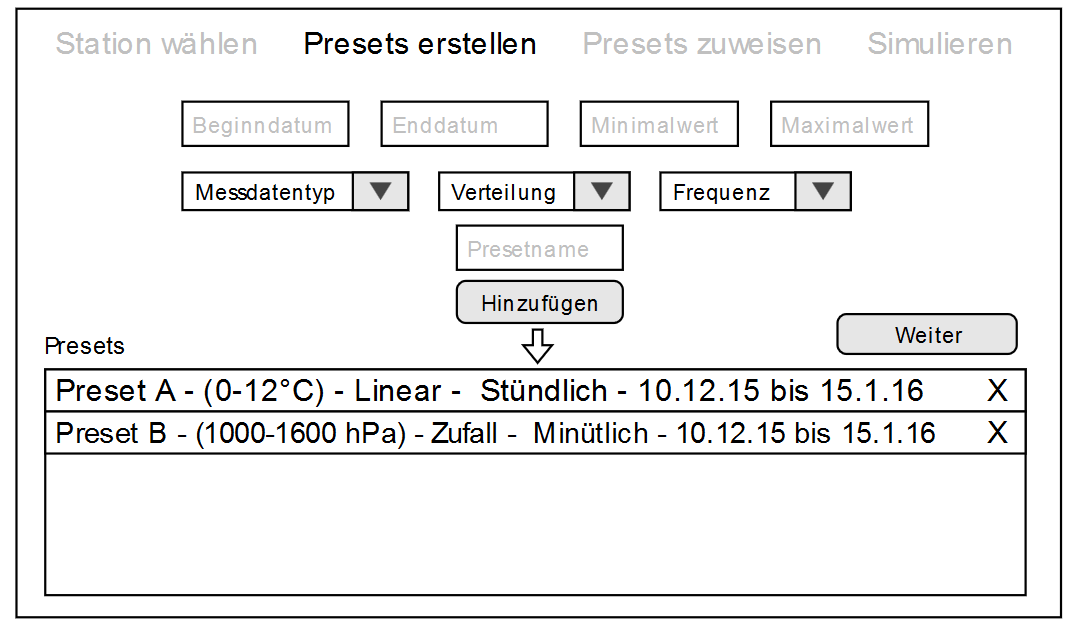
\includegraphics[width=1\textwidth]{pictures/sketches/simulator/add_presets.png}
\caption{UI Sketch für das Erstellen von Presets}
\label{fig:sketch_add_preset}
\end{figure}
\raggedright

\newpage

\subsubsection{Presets zu Stationen zuweisen}

In diesem Schritt können den einzelnen Stationen beliebig viele Presets zugewiesen werden. In Abbildung \ref{fig:sketch_assign_preset} ist zu sehen, dass per Klick auf die Station in der linken Spalte sich der Text über der mittleren Spalte ändert, damit deutlich wird, dass nun Presets zur Station B zugewiesen werden können. Das Zuweisen bzw. Löschen von Presets für die ausgewählte Station funktioniert gleich wie im ersten Schritt beschrieben. Per Klicken auf einen Eintrag der rechten Spalte, wird dieser in die mittlere Spalte verschoben und umgekehrt. Die Pfeile dienen wieder zur Verdeutlichung der gewünschten Interaktion der beiden Spalten.

\begin{figure}[H]
\centering
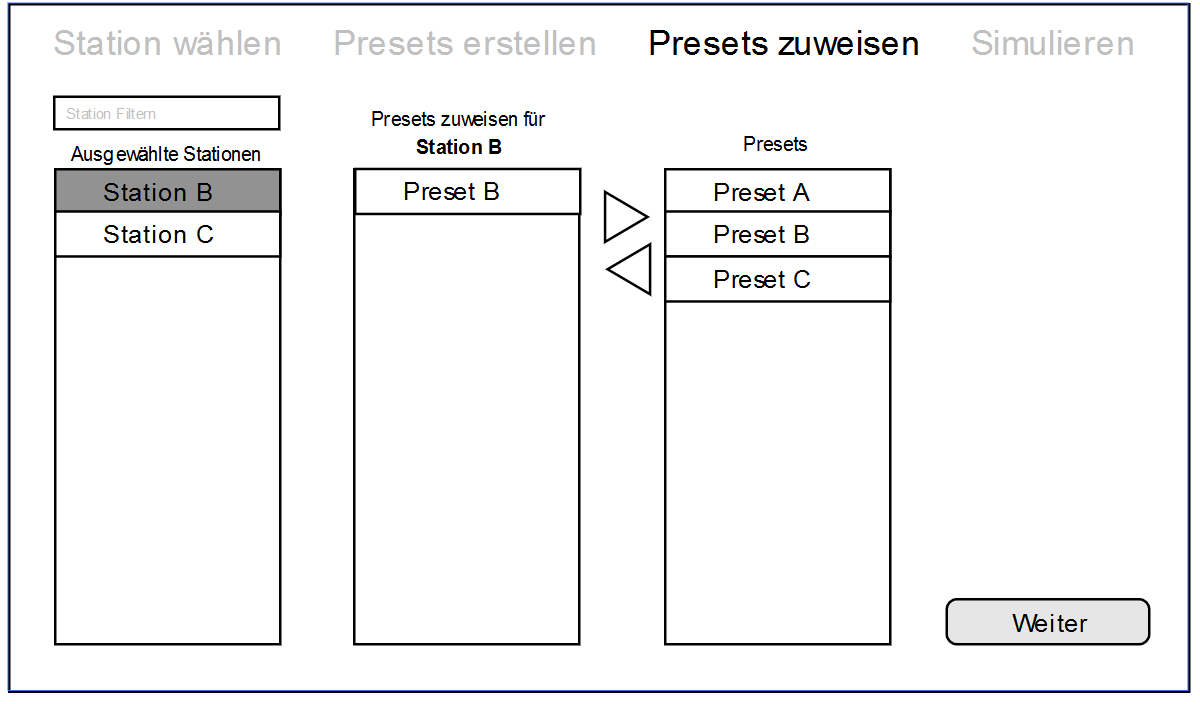
\includegraphics[width=1\textwidth]{pictures/sketches/simulator/assign_preset.png}
\caption{UI Sketch für das Zuweisen von Presets zu Stationen}
\label{fig:sketch_assign_preset}
\end{figure}
\raggedright

\newpage

\subsubsection{Simulationsübersicht}

Abbildung \ref{fig:sketch_simulation} zeigt die Liveansicht des Simulators in dem mit den zwei Buttons die Simulation gestartet oder gestoppt werden kann. Die Geschwindigkeit der Simulation, kann mit dem Slider zwischen Echtzeit und einem Vielfachen davon angepasst werden. Um bei hoher Last die Simulation zu entlasten, kann mit der Checkbox \glqq Graphen berechnen\grqq\ die Live-Visualisierung deaktiviert werden. Ansonsten wird pro in der rechten Dropdownliste ausgewählten Station für jedes zugewiesene Preset ein Graph gezeichnet, der den Verlauf der generierten Messdaten darstellt. Rechts davon befindet sich eine Liste der zugewiesenen Presets, die deaktiviert werden können, um die Visualisierung übersichtlicher zu gestellten.

\begin{figure}[H]
\centering
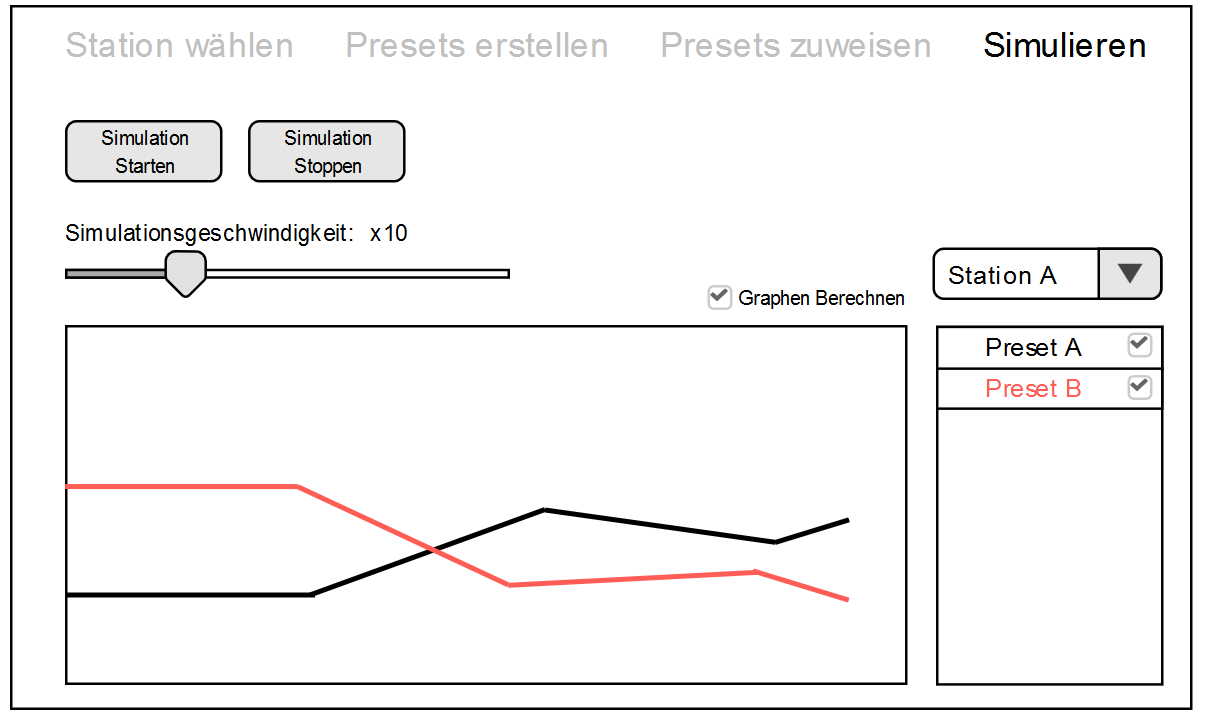
\includegraphics[width=1\textwidth]{pictures/sketches/simulator/simulate.png}
\caption{UI Sketch für die Simulationsübersicht}
\label{fig:sketch_simulation}
\end{figure}
\raggedright


\newpage

\subsection{Cockpit}

Das Cockpit besteht im wesentlichen aus drei Komponenten, welche über die linke Sidebar erreichbar sind.
\begin{itemize}
    \item Home/Dashbaord - Zeigt allgemeine Informationen und eine Wochenübericht an
    \item Analysis - Hier können komplexe Wetterabfragen getätigt werden
    \item Stationen - Verwalten der eigenen Stationen
\end{itemize}

\subsection{Login}

Die Loginmaske ist wie in Abbildung \ref{fig:cock_login} zu sehen sehr einfach gehalten. Es gibt zwei Felder, eines für die Email Adresse und eines für das Passwort. Mit dem Drücken des Login Buttons werden die eigen ebenen Daten validiert, und die anderen Bereiche freigeschaltet. Es wird automatisch auf den Homescreen bzw. das Dashboard umgeleitet.

\begin{figure}[H]
\centering
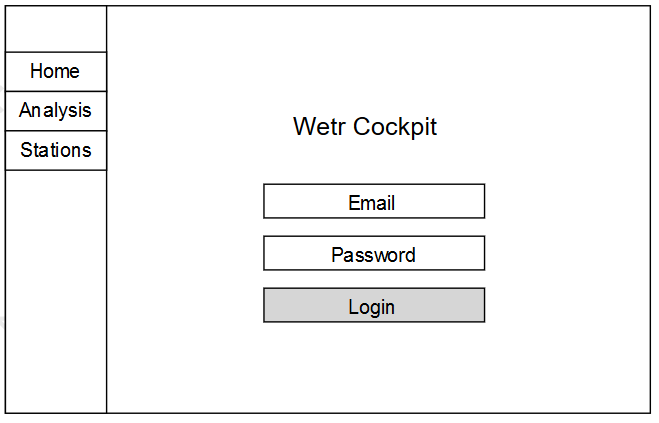
\includegraphics[width=1\textwidth]{pictures/sketches/cockpit/cockpit_login.png}
\caption{UI Sketch für die Loginmaske}
\label{fig:cock_login}
\end{figure}
\raggedright
\newpage
\subsection{Dashboard}

Hier werden allgemeine Informationen über das System (Anzahl der Stationen bzw Messdaten, u.w.) angezeigt. Die Wochenhistory (siehe Abbildung \ref{fig:cock_dash}) zeigt für die einzelnen Seiten die verschiedene Messtypen wie Temperatur oder Luftdruck an. Es kann mittels den unteren Knöpfen zwischen den Seiten gewechselt werden.

\begin{figure}[H]
\centering
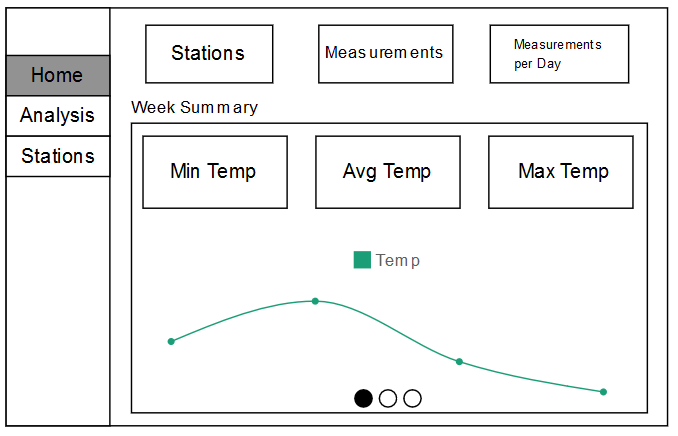
\includegraphics[width=1\textwidth]{pictures/sketches/cockpit/cockpit_home.png}
\caption{UI Sketch für das Dashboard}
\label{fig:cock_dash}
\end{figure}
\raggedright
\newpage

\subsection{Anfrage Stellen}
In dieser Ansich kann recht genau angegeben werden, welche Daten abgefragt und dargestellt werden sollen. Zu beginn muss der Typ also Avg, Min oder Max gewählt werden. Die Gruppierung gruppiert die abgefragten Werte nach Tag, Woche oder Monat. Es muss außerdem der Messdatentyp angegeben werden. Danach kann wie in Abbildung \ref{fig:cock_query} zu sehen die Stationen gewählt werden, von denen die Daten verwendet werden solle. Wenn keine Filterung der Stationen durchgeführt wird, werden alle Stationsdaten berücksichtigt. Als letzten Schritt kann der Ort eingeschränkt werden wobei entweder Koordinaten eingegeben werden können oder anhand von bereits existierenden Orten gefiltert werden kann.

\begin{figure}[H]
\centering
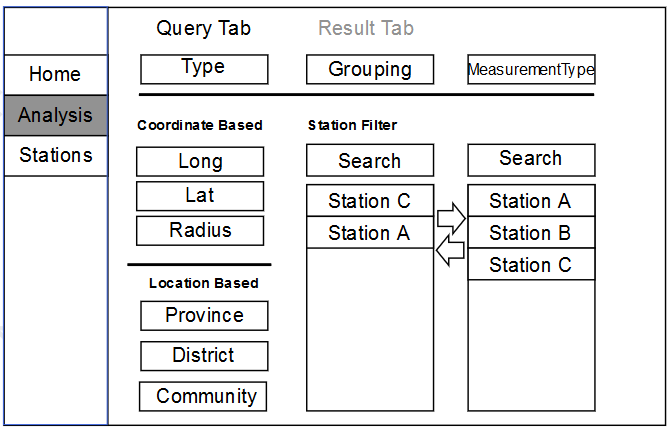
\includegraphics[width=1\textwidth]{pictures/sketches/cockpit/cockpit_query.png}
\caption{UI Sketch für das Eingeben der Abfragedaten}
\label{fig:cock_query}
\end{figure}
\raggedright
\newpage


\subsection{Ergebnis anzeigen}

Das Ergebnis der zuvor abgefragten Daten wird mittels eines Graphen (siehe Abbildung \ref{fig:cock_result}) dargestellt. Werden die Daten im Nachhinein geändert, wird der Graph neu gezeichnet.

\begin{figure}[H]
\centering
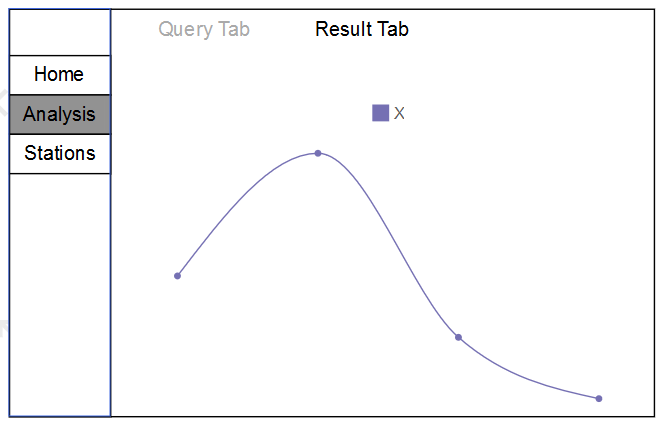
\includegraphics[width=1\textwidth]{pictures/sketches/cockpit/cockpit_result.png}
\caption{UI Sketch für Anzeigen der Resultate}
\label{fig:cock_result}
\end{figure}
\raggedright
\newpage

\subsection{Station bearbeiten}

Die in Abbildung \ref{fig:cock_edit} zeigt die Ansicht zum Editieren von den eigenen Stationen. Hierbei muss um Dropdown-Menü die zu editierende Stationen ausgewählt werden. Danach können die gezeigten Eigenschaften verändert und gespeichert werden. Das Löschen von Stationen ist nur möglich, falls noch keine Messdaten vorhanden sind.

\begin{figure}[H]
\centering
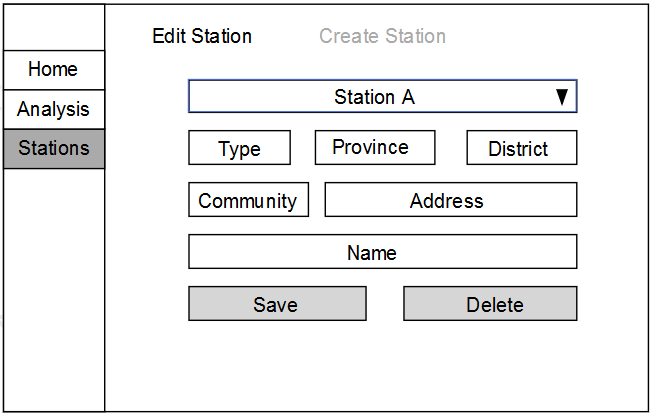
\includegraphics[width=1\textwidth]{pictures/sketches/cockpit/cockpit_edit.png}
\caption{UI Sketch für Bearbeiten der Stationen}
\label{fig:cock_edit}
\end{figure}
\raggedright
\newpage

\subsection{Station erstellen}
Das Erstellen von Stationen läuft nach dem selben Schema. Abbildung \ref{fig:cock_add} zeigt hierbei wieder das Formular mit den auszufüllenden Daten.
\begin{figure}[H]
\centering
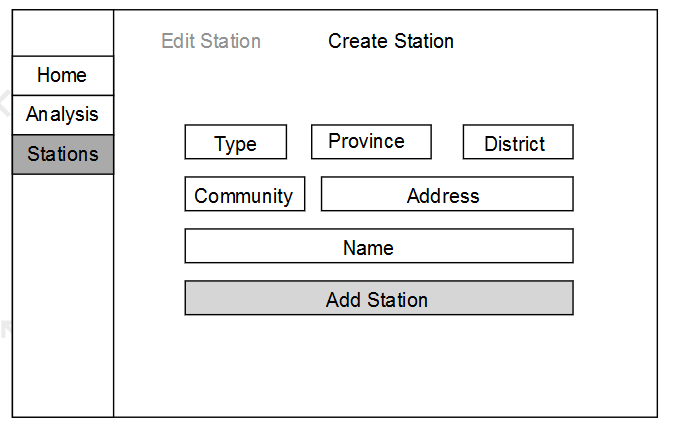
\includegraphics[width=1\textwidth]{pictures/sketches/cockpit/cockpit_create.png}
\caption{UI Sketch für Hinzufügen der Stationen}
\label{fig:cock_add}
\end{figure}
\raggedright
\newpage

\section{Datenbankdesign}

Dieses Projekt wurde mit eines MySQL Datenbank auf Version 5.7.23 realisiert. Es wurden zuerst die geforderten Entitäten aus der Angabe extrahiert und mithilfe eines grafischen Modellierungswerkzeugs namens MySQL Workbench 8\footnote{https://dev.mysql.com/downloads/workbench/} modelliert.

\begin{figure}[H]
\centering
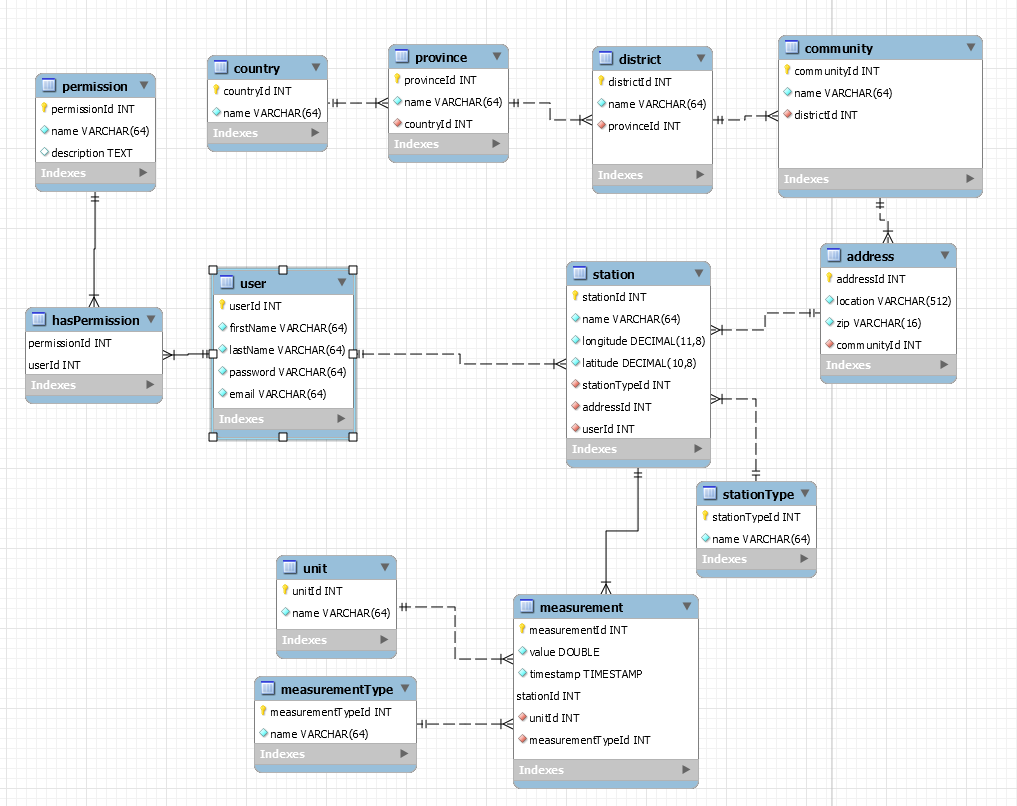
\includegraphics[width=\textwidth]{database.png}
\caption{Datenbankschema des Wetr-Projekts in der ersten Ausbaustufe.}
\label{fig:db}
\end{figure}
\raggedright

Wie in Abbildung \ref{fig:db} zu sehen wird zur Verwaltung des Standortes einer Station eine Reihe von abhängigen Entitäten verwendet. Um die Flexibilität zu erhöhen wurde neben zusätzlich ein \textit{Country} modelliert. In einem \textit{Country} befinden sich \textit{Provinces}, welche Bundesländer darstellen. Jede \textit{Province} wird in mehrere \textit{Districts} unterteilt, ähnlich wie Bezirke. In jedem \textit{District} gibt es mehrere \textit{Communities}, welche mit Gemeinden vergleichbar sind. Als kleinste Entität in dieser Kette gibt es die \textit{Address}, welche einen einfachen String zur Angabe von genaueren Addressdaten (rein zur Anzeige oder falls anderswo benötigt) und eine Zuordnung mittels Postleitzahl enthält.\\
Im Datenbankschema gibt es \textit{User}, welche, falls benötigt, verschiedene \textit{Permissions} zugewiesen haben können. Ein \textit{User} kann mehrere \textit{Stations} betreiben, welche wiederum neben der \textit{Address} auch einen Namen und die Geokoordinaten in Form von Latitide und Longitude gespeichert hat. Der Typ der Station wurde in eine eigene Entität \textit{StationType} ausgelagert.\\
Jede \textit{Station} kann beliebig viele \textit{Measurements} generieren, welche neben den ebenfalls ausgelagerten Entitäten \textit{MeasurementType} und \textit{Unit}, auch einen Zeitstempel und dazugehörigen Messwert besitzen.\\

\subsection{Beispieldaten Generierung}

\subsubsection{Stationen, Addressen und Communities}

Der \textit{Extractor} (befindet sich im extractor Ordner) wurde mit Python\footnote{https://www.python.org/} geschrieben und verwendet die Stationsliste der \textit{Zentralanstalt für Meteorologie und Geodynamik}\footnote{https://www.zamg.ac.at/cms/de/klima/messnetze/wetterstationen}. Die \grqq{}.csv\grqq{} Datei wird vom Extractor eingelesen und für jede \textit{Station} wird eine Insert Anweisung in eine \grqq{}.txt\grqq{} Datei geschrieben. Zusätzlich wird anhand des Längen- und Breitengrades der Ort mit einem geolocator der Aufenthaltsort der Station ermittelt. Anhand dieser Daten werden SQL Anweisungen für die \textit{Community} und \textit{Address} Tabellen erstellt die von der jeweiligen Stationen referenziert werden.

\subsubsection{Messdaten}
Für die erste Ausbaustufe dieses Projekts wurde ein Generator implementiert, der über eine Millionen Messdaten generiert. Diese Messdaten sind jedoch nicht realitätsnahe, sondern haben als Basis den Jahresdurchschnitt in Österreich laut Klimatabelle\footnote{https://www.klimatabelle.info/europa/oesterreich}.
Für eine genauere Beschreibung siehe Abschnitt \ref{sec:generator}.

\subsubsection{Andere Daten}
Die Beispieldaten der restlichen Tabellen wurden per Hand mithilfe vom Internet zusammengestellt. \textit{Provinces}, \textit{Districts} und weiter Standortbezogene Daten sind höchstwarhscheinlich nicht vollständig übernommen worden.

\addtocontents{toc}{\protect\newpage}


\section{Visual Studio Projektmappe}

Das gesamte Projekt befindet sich in einer Visual Studio Projektmappe, welch in folgene Unterprojekte gegliedert ist:
\begin{itemize}
    \item \textbf{Common.Dal.Ado}: Hier befinden sich Hilfsklassen, die den Umgang mit ADO.NET leichter gstalten.
    \item \textbf{Wetr.Domain}: Dieses Projekt beinhaltet die Domainobjekte, welche als einfache Datenbehälter genutzt werden.
    \item \textbf{Wetr.Dal.Interface}: In diesem Paket befinden sich die Interfaces für die Datenzugriffschricht für jedes Domainobjekt bzw. Tabelle.
    \item \textbf{Wetr.Dal.Ado}: Die ADO.NET Implementierung der Datenzugriffsschicht Interfaces.
    \item \textbf{Wetr.Dal.Factory} Beinhaltet Factories um die Instanziierung der benötigen komkreten Klassen zu abstrahieren.
    \item \textbf{Wetr.Test.Dal} Dieses Projekt beinhaltet Unit-Tests für die Datenzugriffsschicht.
    \item \textbf{Wetr.Generator}: Zuständig für das Generieren von Messdaten für die einzelnen Stationen.
    \item \textbf{Wetr.Cockpit.Wpf}: Cockpit Programm, verwendet WPF, MVVM Light Toolkit\footnote{http://www.mvvmlight.net/}, MahAppsMetro\footnote{https://mahapps.com/} und LiveCharts\footnote{https://lvcharts.net/} um Usern die Möglichkeit zu geben Messtationen anzuzeigen bzw ändern zu können.
    \item \textbf{Wetr.Simulator.Wpf}: Simulator Programm, verwendet ebenfalls WPF, MVVM Light Framework, MahAppsMetro und LiveCharts. Hier können Messwerte für Stationen generiert werden.
\end{itemize}

\newpage
\subsection{Common.Dal.Ado}
Das \textit{Common.Dal.Ado} Projekt verwendet die Klassen \textit{AdoTemplate}, \textit{DefaultConnectionFactory}, \textit{IConnectionFactory}, \textit{Parameter} und  \textit{RowMapper}. In der  \textit{AdoTemplate} Klasse werden alle anderen Klassen verwendet. Mithilfe  \textit{IConnection} wird eine Verbindung zu Datenbank aufgebaut.  \textit{AdoTemplate} stellt eine Funktion  \textit{QueryAsync} bereit um eine Datenbankabfragen durchführen zu können.

\begin{figure}[H]
\centering
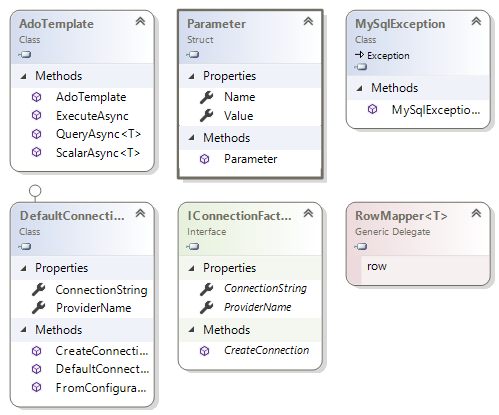
\includegraphics[width=.45\textwidth]{pictures/Common_Dal_Ado_ClassDiagramm.png}
\caption{Common.Dal.Ado UML Diagramm}
\label{fig:common.dal.ado}
\end{figure}
\raggedright

\newpage
\subsection{Wetr.Dal.Interface}
Im \textit{Wetr.Dal.Interface} Projekt wird für jede Klasse in  \textit{Wetr.Domain} ein eigenes Interface bereitgestellt das von den jeweiligen \textit{Dao} Objekten implementiert wird. Jedes Interface implementiert \textit{IDaoBase}$<$\textit{T}$>$. Dieses Interface fasst die Methoden, die in jedem abgeleiteten \textit{Dao Objekt} implementiert werden müssen, zusammen (FindAll, FindById, Delete, Insert, Update).

\begin{figure}[H]
\centering
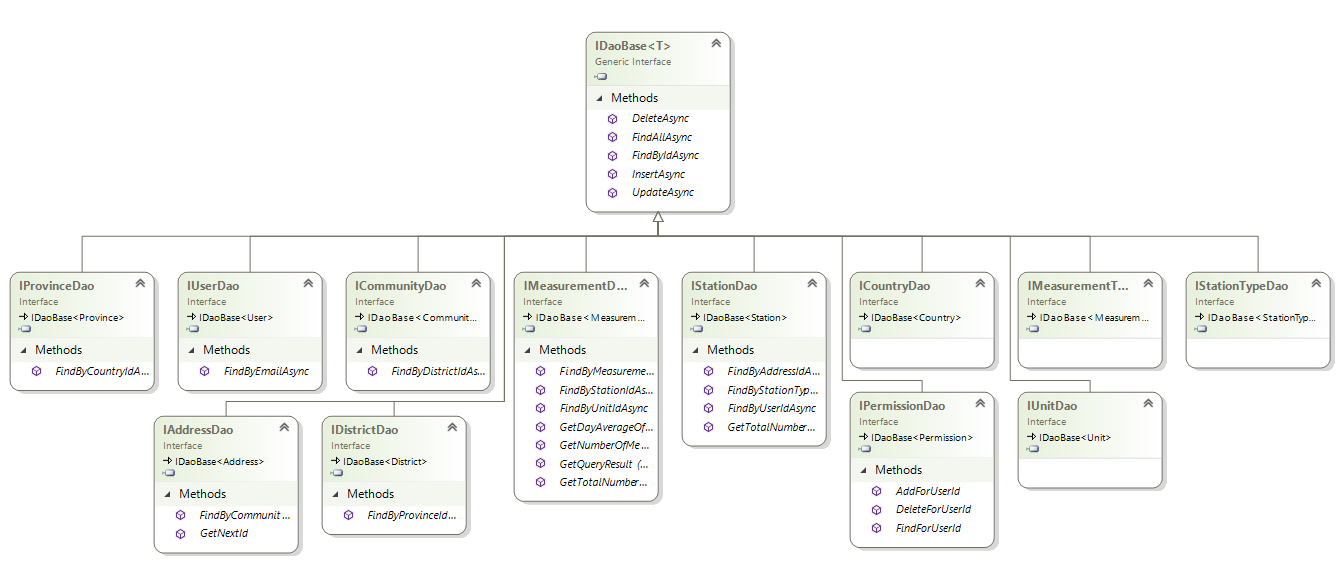
\includegraphics[width=.8\textwidth]{pictures/Wetr_Dal_Interface.png}
\caption{Wetr.Dal.Interface UML Diagramm}
\label{fig:Wetr.Dal.Interface}
\end{figure}
\raggedright

\newpage
\subsection{Wetr.Dal.Ado}
Mit den Klassen im \textit{Wetr.Dal.Ado} Projekt kann eine Verbindung zur Datenbank aufgebaut werden und spezielle SQL Operationen ausgeführt werden. Für jedes \textit{Dao} Objekt gibt es eine \textit{Wetr.Domänen} Klasse. Diese Klassen werden als Behälter Klassen für die angefragten Daten der Datenbank verwendet.

\begin{figure}[H]
\centering
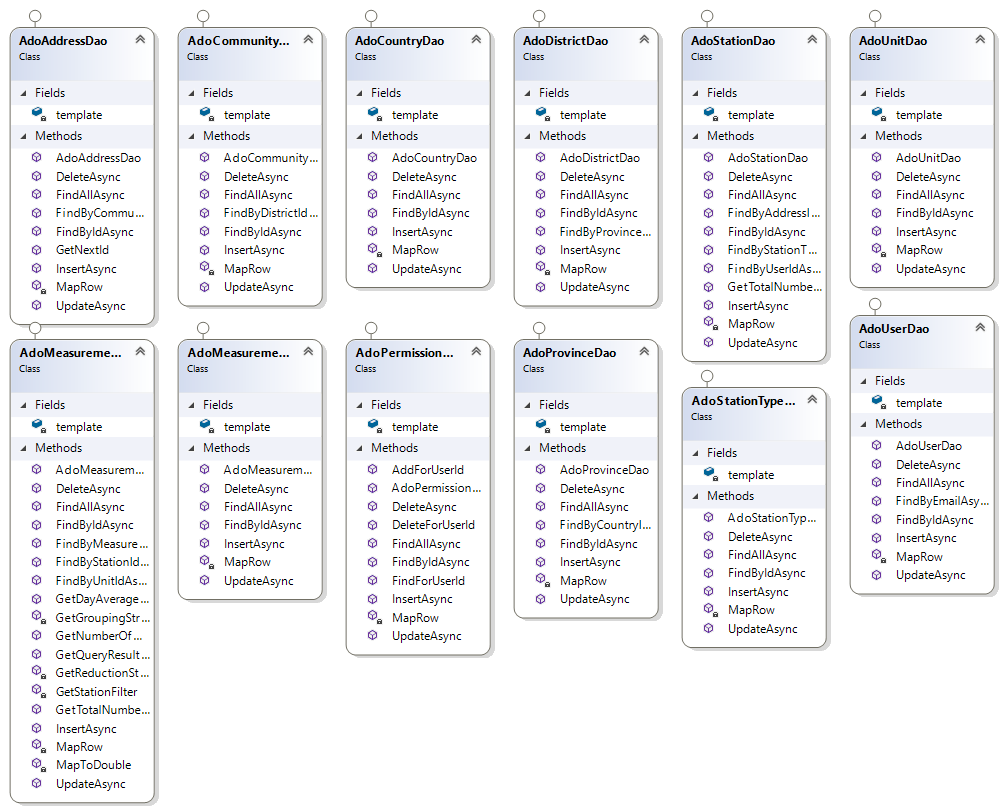
\includegraphics[width=.8\textwidth]{pictures/Wetr_Dal_Ado.png}
\caption{Wetr.Dal.Ado UML Diagramm}
\label{fig:Wetr.Dal.Ado}
\end{figure}
\raggedright

\subsection{Wetr.Dal.Factory}
Im \textit{Wetr.Dal.Factory} Projekt wird eine Klasse \textit{AdoFactory} bereitgestellt mit deren Hilfe ein \textit{Dao} Objekt erstellt werden kann.

\begin{figure}[H]
\centering
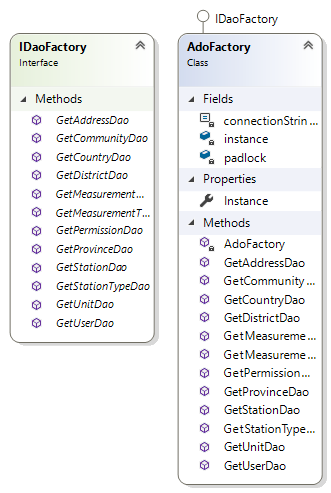
\includegraphics[width=.45\textwidth]{pictures/Wetr_Dal_Factory.png}
\caption{Wetr.Dal.Factory UML Diagramm}
\label{fig:Wetr.Dal.Factory}
\end{figure}
\raggedright

\newpage
\subsection{Wetr.Domain}
Das \textit{Wetr.Domain} Projekt enthält alle Behälterklassen für alle \textit{Dao} Objekte.

\begin{figure}[H]
\centering
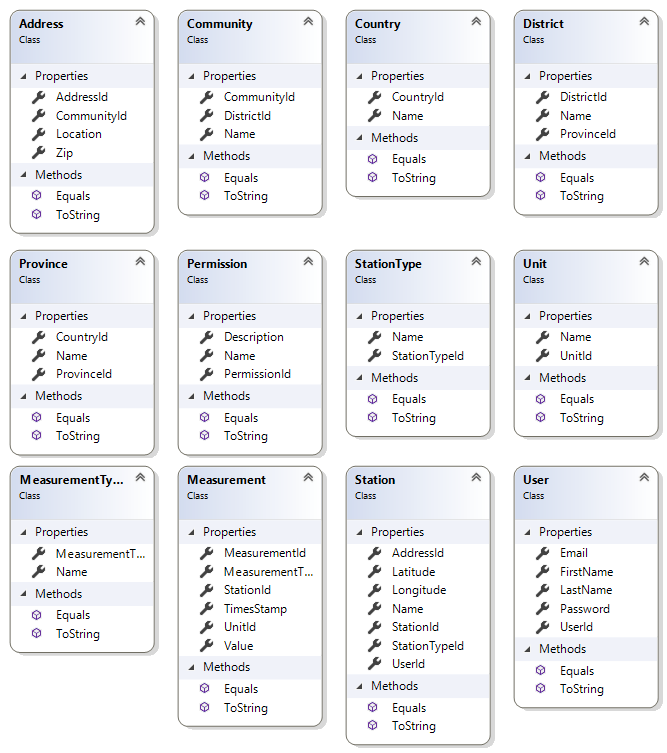
\includegraphics[width=.8\textwidth]{pictures/Wetr_Domain.png}
\caption{Wetr.Domain UML Diagramm}
\label{fig:Wetr.Domain}
\end{figure}
\raggedright

\newpage
\subsection{Wetr.Test.Dal}
Beim \textit{Wetr.Test.Dal} Projekt werden alle Funktionen von jedem \textit{Dao} Objekt getestet. Alle Tests wurden von der Klassen DaoBaseTest abgeleitet, welche Test für Dao-Methoden forcieren, welche in allen Daos implementiert wurden. 

\begin{figure}[H]
\centering
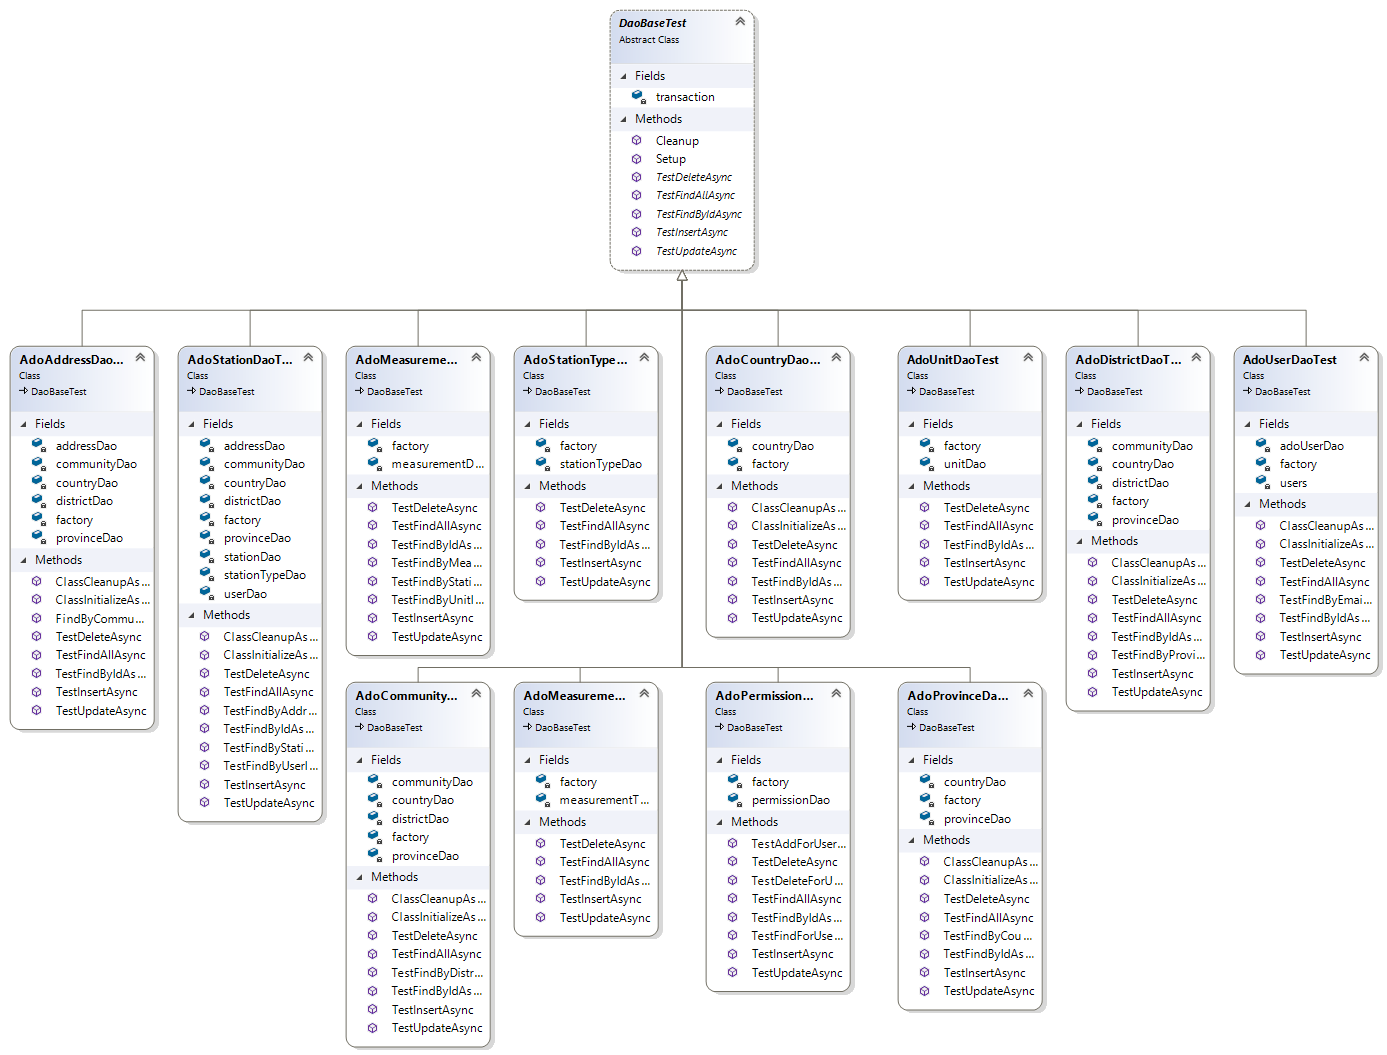
\includegraphics[width=.8\textwidth]{pictures/Wetr_Test_Dal.png}
\caption{Wetr.Domain UML Diagramm}
\label{fig:Wetr.Test.Dal}
\end{figure}
\raggedright

\begin{figure}[H]
\centering
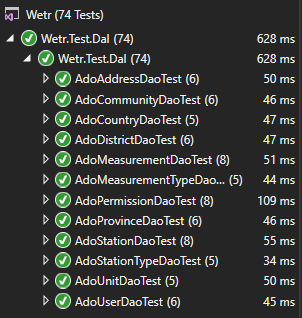
\includegraphics[width=.4\textwidth]{pictures/green_tests.png}
\caption{Beweis, dass die UnitTests erfolgreich durchlaufen.}
\label{fig:Wetr.Test.Dal}
\end{figure}
\raggedright

\newpage
\subsection{Wetr.Generator}
\label{sec:generator}

Der Generator generiert pro \textit{MeasurementType} eine eigene Datei, in der sich die generierten Messdaten befinden. Pro Typ werden nicht genau gleich viele Messdaten generiert, somit ergibt sich eine Summe von etwa 1.2 Millionen Messdaten. Das Format der erzeugten Dateien ist so gestaltet, damit es mit einem speziellen SQL Befehl mittels Bulk-Insert\footnote{https://stackoverflow.com/questions/14330314/bulk-insert-in-mysql} sehr schnell in die Datenbank aufgenommen werden kann. Die generierten Daten haben einen Zeitstempel, der sich innerhalb von einem Jahr bewegt.~\\~\\ %WTF LaTeX?

\textbf{Temperatur}\\
Es wird jede Stunde ein Messwert generiert, der je nach Jahreszeit die Temperatur nach natürlichem Verlauf, sprich zur Mittagszeit ist es am wärmste und in der Nacht am kältesten, gestaltet. Die Werte beinhalten eine zufällige Abweichung von $\pm 1.25$. Der Minimal- bzw. Maximalwert wird pro Jahreszeit nach klimatabelle.info festgelegt.~\\~\\ %WTF LaTeX?

\textbf{Luftfeuchtigkeit}\\
Die Berechnung der Luftfeuchtigkeit funktioniert gleich, wie die der Temperatur, nur, dass die durchschnittlichen Luftfeuchtigkeitswerte hergenommen wurden. Als zufällige Abweichung wurden $\pm10\%$ gewählt.~\\~\\ %WTF LaTeX?

\textbf{Niederschlag}\\
Da nur der jährliche Durchschnittsniederschlag pro Jahreszeit zur Verfügung stand, wurden nicht stündlich, sondern täglich ein Messert generiert. Dieser Wert bewegt sich zwischen $0$ und der Anzahl des durchschnittlichen Tagesniederschalag Mal zwei.~\\~\\ %WTF LaTeX?

\textbf{Luftdruck}\\
Jede Stunde wird ein Luftdruckwert generiert, der zufällig zwischen $900$ und $1100$ Hektopascal liegt.~\\~\\ %WTF LaTeX?

\textbf{Windrichtung}\\
Die Windrichtung ändert sich in dieser einfachen Simulation jede Stunde und kann von $0$ bis $360$ Grad betragen.~\\~\\ %WTF LaTeX?

\textbf{Windstärke}\\
Die Generierung der Windstärke ist in der aktuellen Ausbaustufe sehr primitiv gehalten und ändert sich stündlich zufällig von $0$ und $20\ km/h$


\newpage
\subsection{Wetr.Cockpit.Wpf}
Das \textit{Wetr.Cockpit.Wpf} Projekt wird nach dem MVVM Prinzip erstellt.\textit{Views} und \textit{ViewModels} werden verwendet und mithilfe von \textit{DataBinding} werden vom \textit{ViewModel} Daten bei der \textit{View} angezeigt. Nach dem erfolgreichen Login bietet das Cockpit Usern die Möglichkeit Messtationen zu editieren bzw hinzuzufügen. Im weiteren ist es dem User auch möglich die Messwerte seiner Stationen zu aggregieren.
\newline
\newline
Das Hauptprogramm (nach dem Login) ist in drei verschiedenen Tabs eingeteilt: \newline\textit{Home}, \textit{Analysis} und \textit{Stations}.
\newline
\newline
\textbf{Home}\newline
Eine kleine Übersicht über die Stationen des Users. Hier werden nützliche Werte für den User angezeigt (zb. Stationene Anzahl).
\newline
\newline
\textbf{Analysis}\newline
Hier wird die Aggregation der Messwerte der Stationen ermöglicht. Einzelne Stationen und verschiedene Messwertarten können zum Aggregieren ausgewählt werden.
\newline
\newline
\textbf{Stations}\newline
Im Tab Stations wird dem User die Möglichkeit geboten seine Stationen zu ändern oder neue Stationen hinzuzufügen.

\newpage
\subsection{Wetr.Simulator.Wpf}
Auch dieses Projekt wurde nach dem MVVM Prinzip erstellt.
Der Simulator ist in 4 verschieden Bereiche unterteilt: \textit{Station selection}, \textit{Preset creation}, \textit{Preset assignment} und \textit{Simulation}.
\newline
\newline
\textbf{Station selection}\newline
In diesem Bereich werden die Stationen ausgewählt die für die nachfolgenden Schritte verwendet werden.

\begin{figure}[H]
\centering
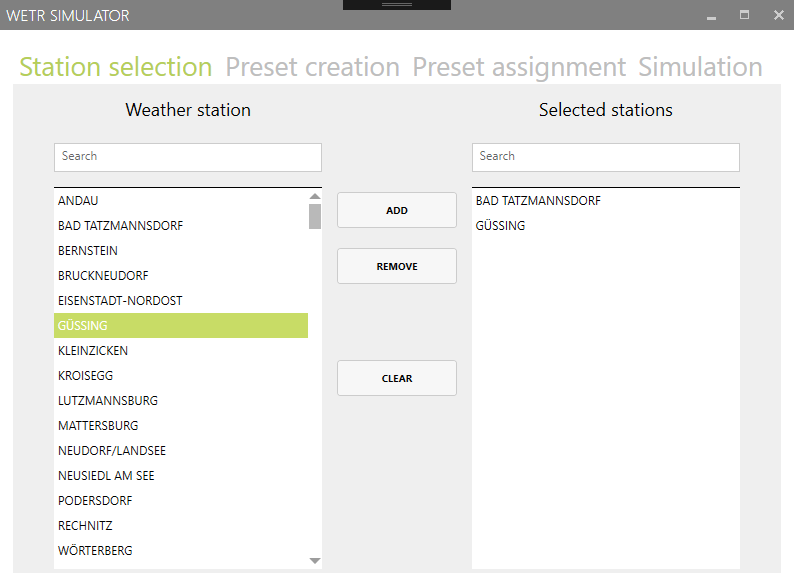
\includegraphics[width=.6\textwidth]{pictures/Simulator/Simulator_1_StationSelection.png}
\caption{Station selection}
\label{fig:Wetr.Simulator.Wpf.StationSelection}
\end{figure}
\raggedright

\textbf{Preset creation}\newline
Ein \textit{Preset} ist eine Berechnungseinstellung. Für diese Einstellung können Daten wie Messart, Start und Enddatum, Minimum und Maximum der Berechnung, Berechnungsart (zb. Linear) und die Regelmäßigkeit der Berechnung eingestellt werden. 
Grundsätzlich können mehrere \textit{Presets} erstellt werden. Diese werden durch den vergebenen Namen identifiziert.

\begin{figure}[H]
\centering
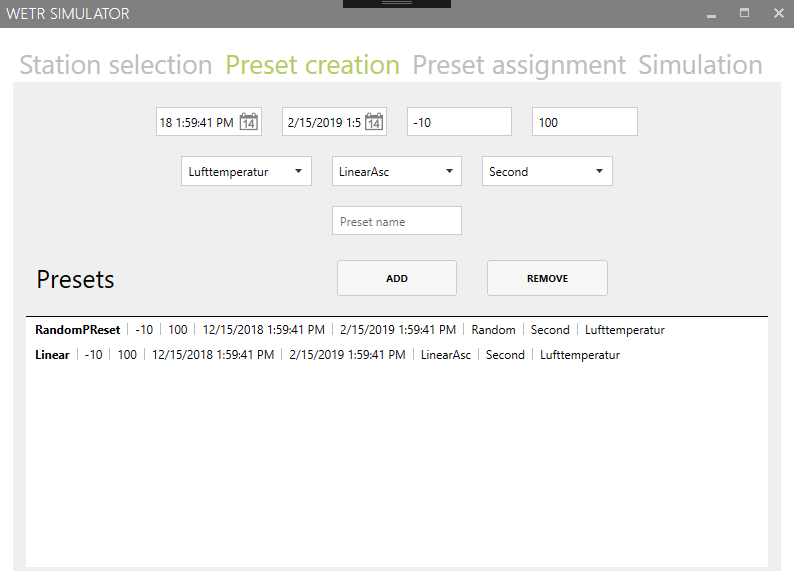
\includegraphics[width=.6\textwidth]{pictures/Simulator/Simulator_2_PresetCreation.png}
\caption{Preset creation}
\label{fig:Wetr.Simulator.Wpf.PresetCreation}
\end{figure}
\raggedright

\textbf{Preset assignment}\newline
Nachdem ein \textit{Preset} erstellt wurde kann diesem eine \textit{Station} zugeteilt werden. Nur \textit{Stationen} die am Anfang ausgewählt wurden können hinzugefügt werden.

\begin{figure}[H]
\centering
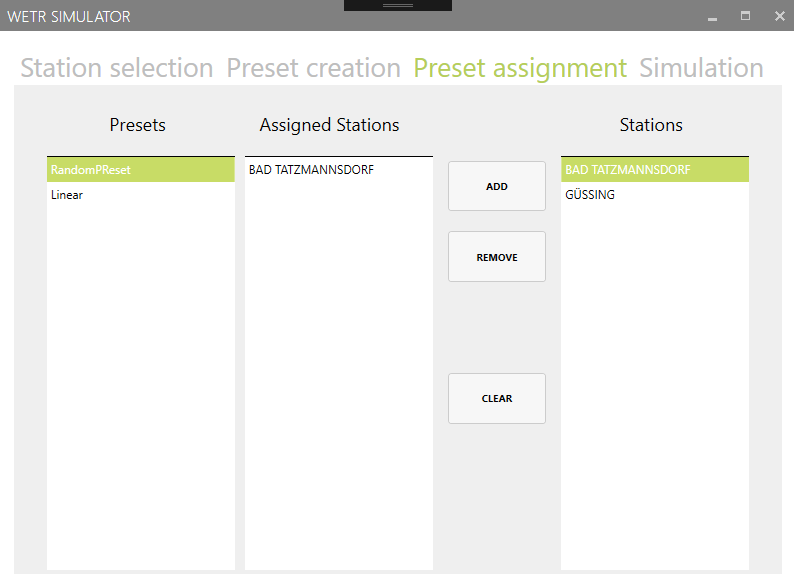
\includegraphics[width=.6\textwidth]{pictures/Simulator/Simulator_3_PresetAssignment.png}
\caption{Preset assignment}
\label{fig:Wetr.Simulator.Wpf.PresetAssignment}
\end{figure}
\raggedright

\textbf{Simulation}\newline
In diesem Bereich können nun die zuvor erstellen \textit{Presets} simuliert werden. Durch auswählen eines \textit{Presets} und anschließendem Starten der Simulation können die Zwischenergebnisse in dem Graphen daneben angezeigt werden. 
Falls die Geschwindigkeit einer Simulation zu langsam ist kann diese mit dem Schieber über dem Graphen verändert werden.

\begin{figure}[H]
\centering
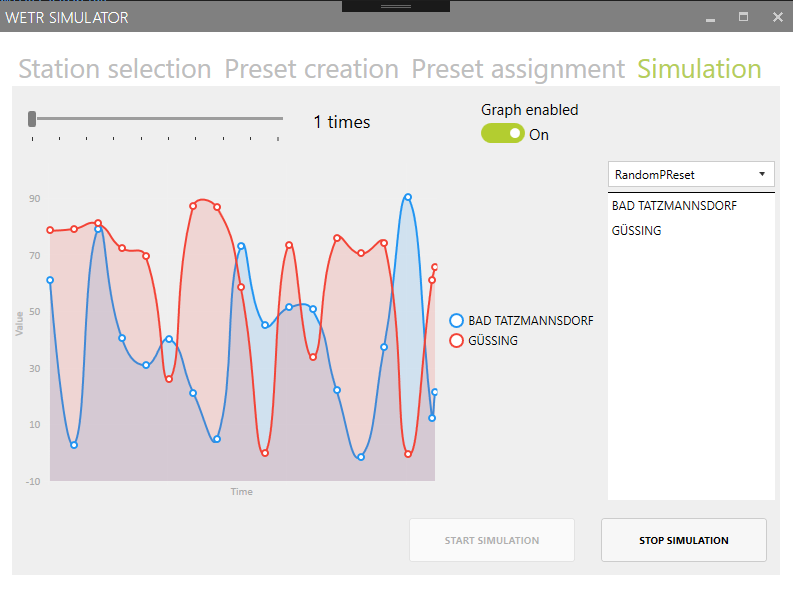
\includegraphics[width=.6\textwidth]{pictures/Simulator/Simulator_4_Simulation.png}
\caption{Simulation}
\label{fig:Wetr.Simulator.Wpf.Simulation}
\end{figure}
\raggedright

\section{REST-API}
\label{rest}

\subsection{Übersicht}

Nur die für WEA5 notwendigen API-Endpunkte wurden implementiert. Diese Funktionalität beinhaltet:
\begin{itemize}
    \item Abfragen statischer Daten (Communitiers, StationTypes, etc.)
    \item Abfragen, Hinzufügen und Ändern von Stationsdaten
    \item Abfragen und Hinzufügen von Messdaten
    \item Authentifizierung mit Benutzerdaten
\end{itemize}

\subsection{Security}

Für die Absicherung von Backend-Routen wurde die JWT-Technologie verwendet.
Beim erfolgreichen Einloggen wird ein Token generiert, der neben dem Ablaufdatum die BenutzerId beinhaltet. Jedes mal, wenn auf eine abgesicherte Route zugegriffen wird, wird der Token entschlüsselt und das Ablaufdatum überprüft. Ist der Token ungültig, wird der Statuscode 401 zurückgesendet.\\

Die im Token enkodierte BenutzerId wird verwendet, um zu überprüfen, ob der Benutzer, der die Anfrage sendet, die benötigten Rechte für die angeforderte Operation hat-

\subsection{Model Validation}
Die Empfangenen Daten werden anhand einfache Regeln wie \textit{required} oder \textit{Range(x,y)} überprüft. Wenn sich Fehler ergeben werden diese als Dictionary, wobei der Schlüssel der Name des fehlerhaften Feldes ist und die Daten ein Array an Fehlermeldung ist.

\subsection{Dokumentation}
Beim Starten vom Projekt \textit{Wetr.Web} wird die REST-Api am lokalen IIS Express ausgeführt. Wenn man zu \textit{http://localhost/5000/swagger} navigiert, wird die Swagger-API-Dokumentation angezeigt.


\section{Anwendungsfälle}
\subsection{Sequenzdiagramm Simulator}

\begin{figure}[H]
\centering
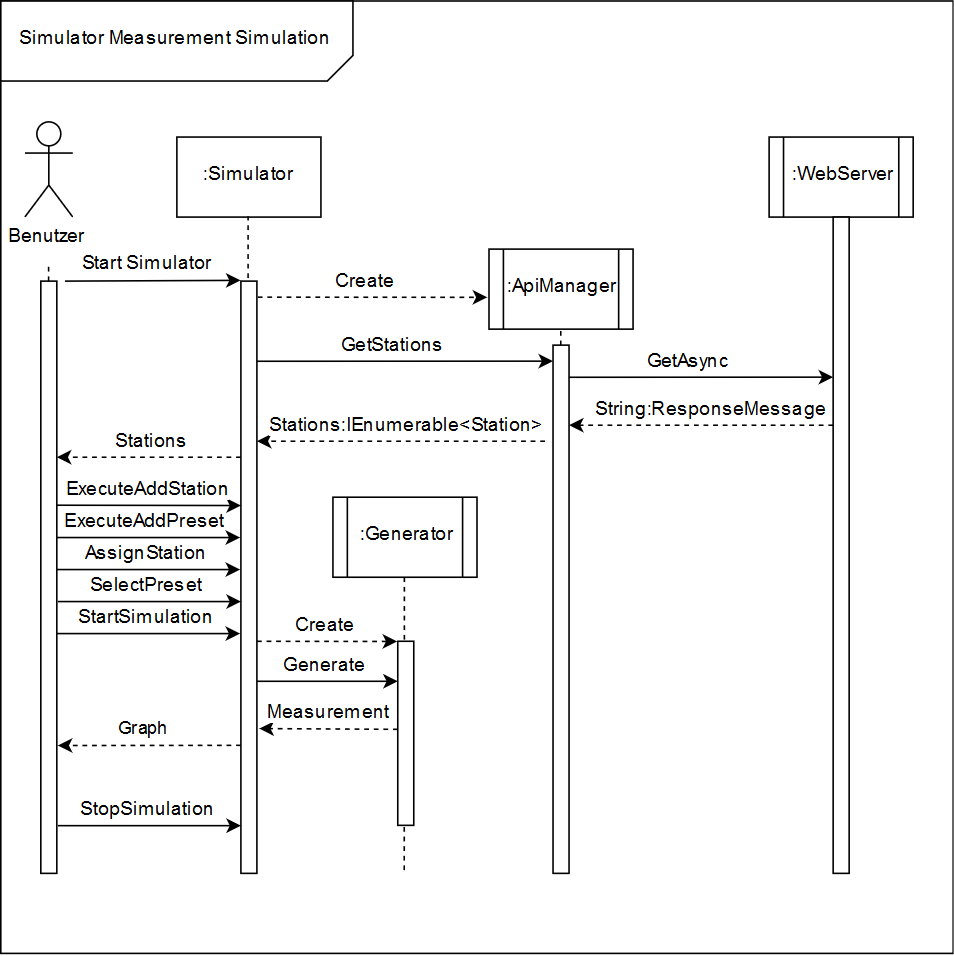
\includegraphics[scale=0.4]{pictures/sequence/Sequence_simulator_full.png}
\caption{Sequenz Diagramm Simulator}
\label{fig:Wetr.Simulator.Wpf-sequence}
\end{figure}
\raggedright

\subsubsection{Beschreibung}
Dem Anwender werden beim Start des Simulators alle verfügbaren Stationen angezeigt die zuvor mithilfe des \textit{ApiManager} geladen wurden. Der \textit{ApiManager} schickt einen request an den Webserver und liefert die Stationen an den Simulator zurück. Danach hat der Anwender die Möglichkeit diese Stationen für die Auswahl zu verwenden. Im nächsten Schritt kann der Anwender ein sogenanntes 'Preset' erstellen. Bei einem 'Preset' kann der Anwender festlegen welche Messwerte simuliert werden sollen und kann die Stationen die diese simulierten Messwerte erhalten bestimmen. Als letzten Schritt kann der Anwender die Simulation mit einem ausgewählten Preset starten oder stoppen. Der \textit{Generator} schickt dabei die generierten Daten mithilfe des \textit{ApiManager} Messwerte an den Webserver.


\newpage

\subsection{Sequenzdiagramm Cockpit}


\begin{figure}[H]
\centering
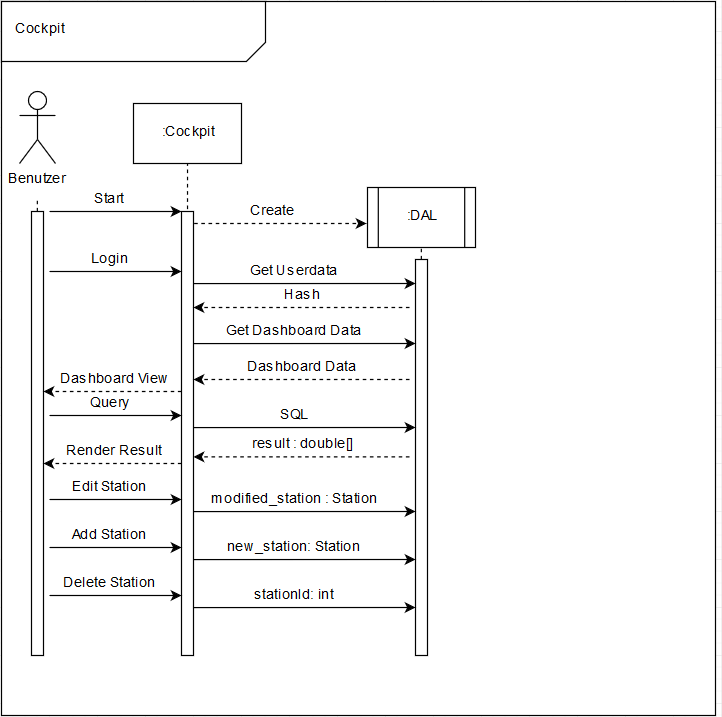
\includegraphics[scale=1.2]{pictures/sequence/Sequence_cockpit_full.png}
\caption{Sequenz Diagramm Cockpit}
\label{fig:Wetr.Cockpit.Wpf-sequence}
\end{figure}
\raggedright

\subsubsection{Beschreibung}

Beim Start des Cockpits muss sich der Benutzer zuerst mit den Benutzerdaten einloggen. Daraufhin frägt die Business Logic des Cockpits den Passworthash ab um ihn zu vergleichen. Bei erfolgreichem Einloggen werden diverse Daten abgefragt, wie z.B Anzahl der Stationen und Messdateb bzw. Wochenrückblick für Temperatur und Regenmenge. Diese Daten werden im Dashboard angezeigt. Wenn der Benutzer eine Messdatenabfrage tätigt, wird diese in einen SQL-String umgewandelt und im Data Access Layer ausgeführt. Das Ergebnis wird in einem Chart angezeigt. Beim Erstellen bzw. Löschen einer Station wird die neue/geänderte Station an den DAL geschickt und dort persistiert. Wenn eine Station gelöscht werden soll, reich es aus, die StationId zu schicken.
\section{Installationsanleitung}

\subsection{Benötigte Programme und Voraussetzungen}
Für dieses Projekt wird zusätzliche Software benötigt:
\begin{itemize}
\item Docker \footnote{https://www.docker.com/}
\item Visual Studio \footnote{https://visualstudio.microsoft.com/de/}
\item MySql-Connector (optional, nur falls notwendig) \footnote{https://dev.mysql.com/get/Downloads/Connector-Net/mysql-connector-net-8.0.13.msi}
\end{itemize}
\raggedright

Um die Datenbank zu erstellen muss Docker gestartet sein. Die Datenbank kann mit dem \textit{Powershell-Script} \grqq{}run.ps1 \grqq{} automatisch generiert werden.
Falls dieses Script wegen fehlender Berechtigungen nicht ausgeführt werden kann, muss eine \textit{Shell} (Git-Bash oder ähnliches) im Ordner mit der Docker Compose Datei \grqq{}docker-compose.yaml \grqq{} geöffnet und folgenden Befehle nacheinander ausgeführt werden:
\begin{minted}{dockerfile}
docker stop $(docker ps -a -q)
docker rm $(docker ps -a -q)
docker-compose up --build --force-recreate
\end{minted}

\subsection{Datenbank}
Für die Datenbank muss die SQL Datei \grqq{}create-wetr.sql \grqq{} im Ordner sql/Create ausgeführt werden. Falls das Unit Testing auch ausgeführt werden soll, wird die zweite SQL Datei \grqq{}create\textunderscore wetr-unit.testing.sql \grqq{} auch benötigt.
\newline\newline
Für die Füllung der Datenbank kann die SQL Datei \grqq{}InsertEverythingWithoutMeasurement.sql\grqq{} verwendet werden. Für die Measurement Daten muss spezieller vorgegangen werden dadurch kann aber die Insert Zeit drastisch verringert werden:
\begin{itemize}
\item Wetr.Generator.exe im Ordner sql/Insert starten
\item http://localhost:8080/ im Browser aufmachen \newline (phpMyAdmin sollte starten)
\item Benutzer: root Passwort: 0c1cd84e
\item Datenbank wetr auswählen
\item Zum SQL Tab wechseln
\item Die nachfolgenden SQL Anweisungen eingeben und ausführen
\end{itemize}
\newpage
\begin{minted}{sql}
LOAD DATA LOCAL INFILE "/tmp/sql/insert/measurementsDownfall.bulk" INTO TABLE measurement
FIELDS TERMINATED BY ', ' ENCLOSED BY "'"
LINES TERMINATED BY '\r\n';

LOAD DATA LOCAL INFILE "/tmp/sql/insert/measurementsHumidity.bulk" INTO TABLE measurement
FIELDS TERMINATED BY ', ' ENCLOSED BY "'"
LINES TERMINATED BY '\r\n';

LOAD DATA LOCAL INFILE "/tmp/sql/insert/measurementsTemperature.bulk" INTO TABLE measurement
FIELDS TERMINATED BY ', ' ENCLOSED BY "'"
LINES TERMINATED BY '\r\n';

LOAD DATA LOCAL INFILE "/tmp/sql/insert/measurementsWind.bulk" INTO TABLE measurement
FIELDS TERMINATED BY ', ' ENCLOSED BY "'"
LINES TERMINATED BY '\r\n';

LOAD DATA LOCAL INFILE "/tmp/sql/insert/measurementsWindDirection.bulk" INTO TABLE measurement
FIELDS TERMINATED BY ', ' ENCLOSED BY "'"
LINES TERMINATED BY '\r\n';

LOAD DATA LOCAL INFILE "/tmp/sql/insert/measurementsPreassure.bulk" INTO TABLE measurement
FIELDS TERMINATED BY ', ' ENCLOSED BY "'"
LINES TERMINATED BY '\r\n';
\end{minted}


\end{document}
